\begin{figure}[H]
	\centering
	% This file was created by matlab2tikz.
%
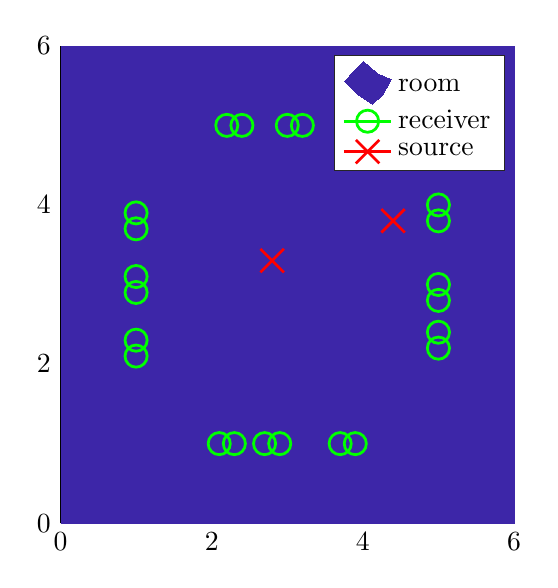
\begin{tikzpicture}

\begin{axis}[%
width=0.475\textwidth,
height=0.5\textwidth,
at={(0\textwidth,0\textwidth)},
scale only axis,
xmin=-0,
xmax=6,
ymin=-0,
ymax=6,
axis background/.style={fill=white},
axis x line*=bottom,
axis y line*=left,
legend style={legend cell align=left, align=left, draw=white!15!black}
]

\addplot[%
surf,
shader=interp, colormap={mymap}{[1pt] rgb(0pt)=(0.239216,0.14902,0.658824); rgb(1pt)=(0.239216,0.14902,0.658824)}, mesh/rows=6]
table[row sep=crcr, point meta=\thisrow{c}] {%
%
x	y	c\\
0	0	0\\
0	1.2	0\\
0	2.4	0\\
0	3.6	0\\
0	4.8	0\\
0	6	0\\
1.2	0	0\\
1.2	1.2	0\\
1.2	2.4	0\\
1.2	3.6	0\\
1.2	4.8	0\\
1.2	6	0\\
2.4	0	0\\
2.4	1.2	0\\
2.4	2.4	0\\
2.4	3.6	0\\
2.4	4.8	0\\
2.4	6	0\\
3.6	0	0\\
3.6	1.2	0\\
3.6	2.4	0\\
3.6	3.6	0\\
3.6	4.8	0\\
3.6	6	0\\
4.8	0	0\\
4.8	1.2	0\\
4.8	2.4	0\\
4.8	3.6	0\\
4.8	4.8	0\\
4.8	6	0\\
6	0	0\\
6	1.2	0\\
6	2.4	0\\
6	3.6	0\\
6	4.8	0\\
6	6	0\\
};
\addlegendentry{room}

\addplot [color=green, line width=1.0pt, draw=none, mark size=4.0pt, mark=o, mark options={solid, green}]
  table[row sep=crcr]{%
2.1	1\\
2.3	1\\
2.7	1\\
2.9	1\\
3.7	1\\
3.9	1\\
5	2.2\\
5	2.4\\
5	2.8\\
5	3\\
5	3.8\\
5	4\\
2.2	5\\
2.4	5\\
3	5\\
3.2	5\\
3.8	5\\
4	5\\
1	2.1\\
1	2.3\\
1	2.9\\
1	3.1\\
1	3.7\\
1	3.9\\
};
\addlegendentry{receiver}

\addplot [color=red, line width=1.0pt, draw=none, mark size=6.0pt, mark=x, mark options={solid, red}]
  table[row sep=crcr]{%
4.4	3.8\\
2.8	3.3\\
};
\addlegendentry{source}

\end{axis}
\end{tikzpicture}%
	\caption{Simulation Setup}
	\label{fig:setup}
\end{figure}

The setup, that is going to be simulated, consists of a rectangular room, that is 6m wide, 6m long and 6m high. There are a total of 12 microphone pairs, 3 of them on each wall. The position of each microphone pair can be seen in Figure~\ref{fig:setup}. The sources are going to be placed within this room with fixed or random positions, depending on the evaluation scenario, and are described using one-dimensional position vectors with x-, y- and z-coordinates (i.e. $\begin{bmatrix} 2&3&3  \end{bmatrix}$ describes a source at the position $x=3, y=3$ and $z=3$)

%\todo{Explain reason for positioning of the microphone pairs}

